% Resultados1
\chapter{Adaptación al control automático del volante} 
\label{chap:volante}

Dado que el sistema se diseñó de la manera más mas genérica posible, se decidió probar el funcionamiento del mismo en el control del volante. El proceso de adaptación consistió en: Ajustar el valor de las variables de entrada que utiliza el sistema, obviar las condiciones correspondientes al cambio de pedal, realizar el cálculo de las variables de entradas asociadas al control del volante y hacer que la modificación de los singletons fuera \textit{simétrica}, ya que las mismas acciones para girar el volante si vamos a agarrar una curva hacia la izquierda, deben ser iguales a las aplicadas para agarrar una curva hacia la derecha, pero con signo contrario.

Utilizamos dos variables de entrada en el controlador, la desviación lateral medida en metros y la variación de la desviación lateral (m/s). En \gls{TORCS} la desviación lateral se calcula con respecto al medio de la pista, en Platero es con respecto a un mapa predefinido, el cual se carga al activar el programa de control automatizado. Ambas variables de entrada fueron limitadas en el rango [-3,3] y fueron inicializadas con 3 etiquetas. Utilizamos 1 m/s como valor de aceleración de confort y una constante de normalización de 100 que fue la misma utilizada para el control del pedal. 

Para el control de los pedales, se había establecido que para representar el cambio de un pedal a otro, se devolvía cero durante tres ejecuciones del sistema; y para evitar ciertos cambios de pedal innecesario, para cada salida cuyo valor absoluto sea menor a 0.02 se devolvía cero. Estos dos casos fueron obviados cuando se establece que el sistema se va a encargar del control del volante.

\section{Pruebas realizadas con TORCS}

Para comprobar el funcionamiento del sistema al hacerse cargo del control del volante, se realizaron pruebas en \gls{TORCS} utilizando la pista \textit{Alpine-1}. Como se puede ver en la figura \ref{fig:alpine} (izquierda), el recorrido realizado, que va desde el punto \textbf{A} hasta el punto \textbf{B}, posee una gran cantidad de curvas, siendo muchas de ellas muy cerradas, lo cual representa una muy buena prueba para demostrar el funcionamiento del sistema. La prueba se realizó dejando al sistema controlar simultáneamente los pedales y el volante, la velocidad del automóvil se colocó a 15 km/h, ya que por cuestiones de seguridad las pruebas con Platero se iban a realizar a una velocidad muy baja, de modo que se hizo la prueba lo más parecida posible a lo que se tenía pensado hacer con Platero.  

\begin{figure}[htb]
\centering
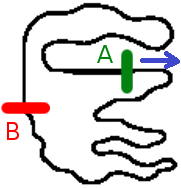
\includegraphics[width=0.2\linewidth]{figures/alpine.PNG}\hspace{0.02\linewidth}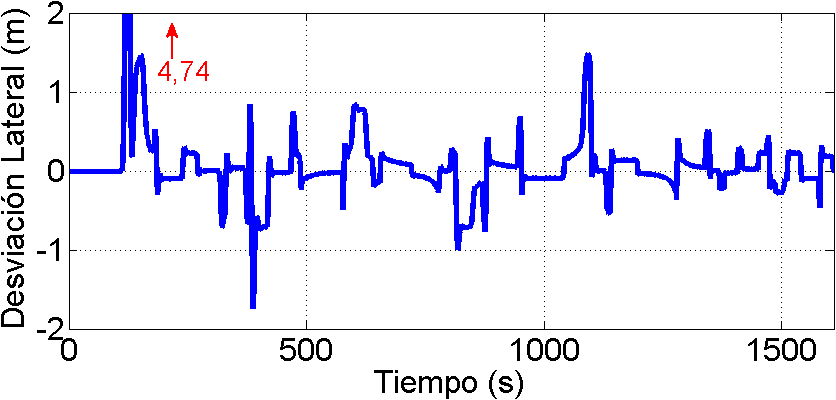
\includegraphics[width=0.6\linewidth]{figures/desvTorcs.png}
\caption{Pista Alpine-1 de TORCS (izquierda). Desviación lateral con respecto al tiempo (derecha).}
\label{fig:alpine}
\end{figure}

Como se puede ver en la figura \ref{fig:alpine} (derecha), que representa la desviación del vehículo con respecto del medio de la pista, se obtuvieron muy buenos resultados. En la primera curva es donde ocurre la mayor diferencia y esto se debe a que en ese instante, los singletons se encontraban todos en cero. Luego de la segunda gran curva, un poco antes del segundo 500, el sistema logró mantener la desviación en el rango [-1,1], hasta que un poco después del instante 1000, toma la última gran curva llegando a una desviación de 1.5, para luego estabilizarse nuevamente y mantener una desviación muy baja.


\section{Pruebas realizadas con vehículo automatizado} 

Utilizando Platero cargamos un mapa que consistió en una vuelta alrededor de \gls{ZOCO}, como se puede apreciar en la figura \ref{fig:zocoV}, y con la misma configuración que se utilizó en la simulación con \gls{TORCS}, se procedió a realizar las pruebas. Por cuestiones de seguridad, el control de los pedales se dejó manual, y se condujo el vehículo a una velocidad aproximada de 10 Km/h; con respecto a la salida del volante, para evitar cambios muy bruscos, se restringió que entre dos salidas consecutivas del controlador la diferencia entre ellas no podía ser mayor a 50 grados.

\begin{figure}[htb]
\centering
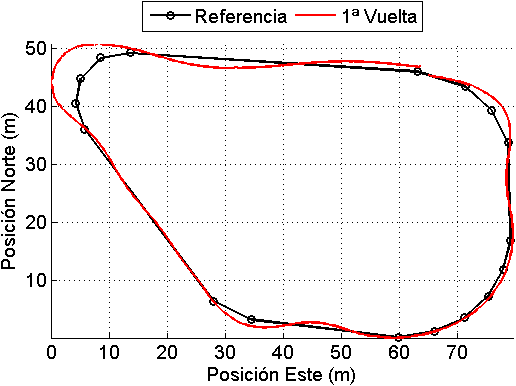
\includegraphics[width=0.48\linewidth]{figures/vuelta1.png}\hspace{0.04\linewidth}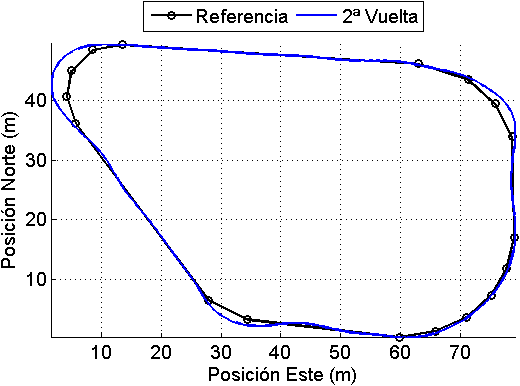
\includegraphics[width=0.48\linewidth]{figures/vuelta2.png}
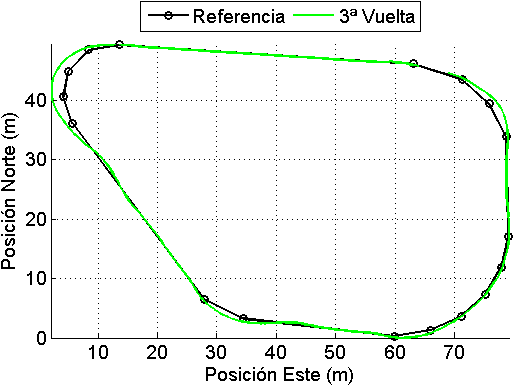
\includegraphics[width=0.5\linewidth]{figures/vuelta3.png}
\caption{Trayectoria del vehículo durante las tres vueltas que se realizaron.}
\label{fig:zocoV}
\end{figure}  

En la figura \ref{fig:desvPlatero} se puede observar como el sistema a medida que fue aprendiendo fue reduciendo la desviación lateral considerablemente, especialmente cuando debía pasar por la primera gran curva, que como se puede ver en la figura \ref{fig:zocoV}, cada vez se tomaba mejor, pasando de una desviación lateral de -5.37 obtenida en la primera vuelta a -2.46 que se obtuvo en la tercera vuelta.   

\begin{figure}[htb]
\centering
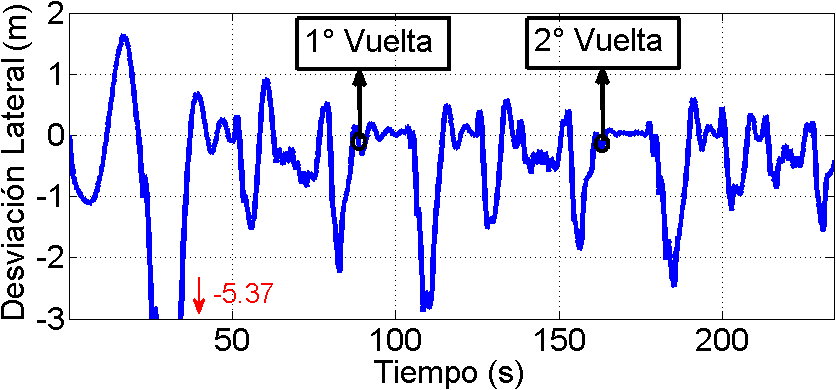
\includegraphics[width=0.8\linewidth]{figures/desviacionPlatero.png}
\caption{Desviación lateral entre el vehículo y el mapa.}
\label{fig:desvPlatero}
\end{figure}

Uno de los inconvenientes que se encontró, fue que como los mapas que se cargaban en Platero para especificar la ruta debían ser construidos a mano especificando las coordenadas de diversos puntos del mapa por los que el vehículo debe pasar, cada vez que se pasaba por uno de esos puntos, el automóvil cambiaba la referencia con respecto a la línea con la cual se calculaba la desviación lateral. Al obtener la desviación con respecto a la nueva referencia, en la mayoría de los casos resultaba que la desviación era muy grande, por lo que obtuvimos ciertos momentos en la prueba donde el volante hacía un movimiento brusco para poder ajustarse a la nueva línea de referencia.